\documentclass{article}
%\documentclass[doc,english]{apa}
\usepackage[utf8]{inputenc}

% packages
\usepackage{amsmath,amsfonts,amssymb, bm}
\usepackage{graphicx,verbatimbox}
\usepackage[colorlinks=true, allcolors=blue]{hyperref}
\usepackage{apacite}
\usepackage{authblk}  % for authors
\usepackage{caption}
%\usepackage{setspace} % doublespacing
\usepackage{subcaption}
\usepackage{booktabs}
\usepackage{nicefrac}

\usepackage{color}
\usepackage{todonotes}



\newcommand{\EJ}[1]{\todo[inline, color=green]{EJ: {#1}}}
\newcommand{\DON}[1]{\todo[inline, color=white]{Don: {#1}}}

\newcommand{\Irater}{r}
\newcommand{\Iitem}{i}
\newcommand{\Ipatient}{p}
\newcommand{\Incat}{c}
\newcommand{\Ilatent}{l}

\newcommand{\Trater}{\expandafter\MakeUppercase\expandafter{\Irater}}
\newcommand{\Titem}{\expandafter\MakeUppercase\expandafter{\Iitem}}
\newcommand{\Tpatient}{\expandafter\MakeUppercase\expandafter{\Ipatient}}
\newcommand{\Tncat}{\expandafter\MakeUppercase\expandafter{\Incat}}
\newcommand{\Tlatent}{\expandafter\MakeUppercase\expandafter{\Ilatent}}

\newcommand{\ilogit}[1]{\text{logit}^{-1}\left(#1\right)}
\newcommand{\dnorm}[2]{\text{Normal}\left(#1,\,#2\right)}
\newcommand{\dgamma}[2]{\text{Gamma}\left(#1,\,#2\right)}

%\newcommand{\dnorm}[2]{\mathcal{N}\left(#1,\,#2\right)}
%\newcommand{\dgamma}[2]{\mathcal{G}\left(#1,\,#2\right)}


\newcommand{\osflink}{\textit{osflink}}

\title{Cultural Consensus Theory for the Evaluation of Patients’ Behavior in Psychiatric  Detention Centers}

\renewcommand{\thefootnote}{\fnsymbol{footnote}}
\author[1]{Don van den Bergh\thanks{Correspondence concerning this article should be addressed to:  
\\  Don van den Bergh 
\\  University of Amsterdam, Department of Psychological Methods
\\  Postbus 15906, 1001 NK Amsterdam, The Netherlands
\\  E-Mail should be sent to: donvdbergh@hotmail.com.}}
\author[1]{wie nog meer?}
\author[1]{Eric-Jan Wagenmakers}
\affil[1]{University of Amsterdam}
\date{}
\renewcommand*{\thefootnote}{\arabic{footnote}}
\begin{document}

\listoftodos
\newpage
\maketitle

\begin{abstract}
In many psychiatric detention centers, patients' mental health is monitored at regular intervals. Typically, clinicians score patients using a Likert scale on multiple criteria including hostility. Having an overview of patients’ scores benefits staff members in at least three ways. First, the scores may help adjust treatment to the individual patient; second, the change in scores over time allow an assessment of treatment effectiveness; third, the scores may warn staff that particular patients are at high risk of turning violent. Practical importance notwithstanding, current practices for the analysis of mental health scores are suboptimal: evaluations from different clinicians are averaged (as if the Likert scale were linear and the clinicians identical), and patients are analyzed in isolation (as if they were independent). Uncertainty estimates of the resulting score are often ignored. Here we outline a quantitative program for the analysis of mental health scores using cultural consensus theory (CCT; \citeNP{Anders2015cultural}). CCT models take into account the ordinal nature of the Likert scale, the individual differences among clinicians, and the possible commonalities between patients. In a simulation, we compare the predictive performance of the CCT model to the current practice of aggregating raw observations and, as a more reasonable alternative, against often-used machine learning toolboxes. In addition, we outline the substantive conclusions afforded by application of the CCT model. We end with recommendations for clinical practitioners who wish to apply CCT in their own work. 
\end{abstract}

\newpage

% Introduction

Psychiatric detention centers monitor the mental health of their patients at regular intervals. A clinician, psychiatrist, or other staff member, henceforth a \textit{rater}, scores a patient on multiple criteria. For example, a rater evaluates a patient's behavior on a variety of criteria that relate to aggressiveness. Next, these ratings of patients' mental health are used for a multiple purposes. For instance, the scores may to help adjust treatment to individual patients; second, the change in scores over time allows for an assessment of treatment effectiveness; third, the scores may warn staff that particular patients are at high risk of turning violent. Moreover, these ratings are key to a quantitative approach of monitoring and predicting patients' behavior.

Current practices for aggregating the scores are suboptimal. Evaluations from different raters are averaged, as if they are exchangeable. For example, personal communication with staff of a psychiatric detention center suggested that clinicians are more lenient in their ratings than psychiatrist, but this information is not used to weigh their ratings. Furthermore, different patients are analyzed in isolation, as if they are independent. Any information regarding a patient's criminal offense is not accounted for in a model-based manner. In addition, any uncertainty estimates of the resulting score are usually ignored. \DON{lookup quote}

An appropriate model for these data captures individual differences among the patients, raters, and items. Cultural Consensus Theory (CCT) is an ideal starting point for such a model, as CCT is designed to pool information from different raters and items \cite{romney1986culture, batchelder1988test, batchelder2012cultural}. The CCT model can be applied to both continuous as well as ordinal  describe raters and items using a hierarchical structure, which allows 

Here we outline a quantitative program for the analysis of mental health scores using CCT. First, a CCT model for ordinal data is introduced \cite{Anders2015cultural}. Afterwards, this model is expanded step by step, in order to include more characteristics of the data. In a simulation, we compare the predictive performance of the CCT model to the current practice of aggregating raw observations and, as a more reasonable alternative, against often-used machine learning toolboxes such as Random Forest \cite{breiman2001random} and Boosted Regression Trees \cite{friedman2002stochastic}. We showcase the substantive conclusions obtained from applying the CCT model and conclude the paper with recommendations for clinical practitioners who wish to apply CCT in their work.

\section*{Cultural Consensus Theory}
\DON{Is het leuk om een korte historische context the geven? Persoonlijk boeit dat mij meestal niet maar sommige lezers zouden het leuk kunnen vinden.}
Historically, CCT used in context of questionnaires where the `true' answers are unknown and estimated from the data. Examples: ``unknown answer key'', political questionnaire.

In the sections below, first a vanilla CCT model is introduced, which is then expanded.


As a starting point, consider the Latent Truth Rater Model cultural consensus model for ordinal data (LTRM) as introduced by \citeA{Anders2015cultural}. We use a model for ordinal data as ratings are generally given on a Likert scale, but CCT can be applied to continuous data as well \cite<e.g., the LTM;>{batchelder2012cultural}. A graphical model of the LTRM is shown in Figure~\ref{model:CCTO}. The LTRM captures differences among raters and items, and may be viewed as the simplest model for a single patient. 
\begin{figure}[!ht]
%	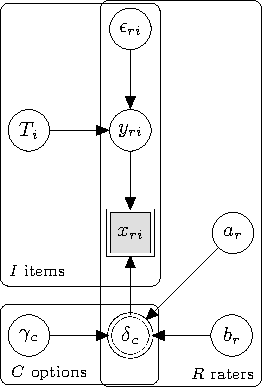
\includegraphics[width=.4\textwidth, page=1]{graphicalModels/graphicalModels.pdf}
	\begin{minipage}{0.5\textwidth}
		\centering
		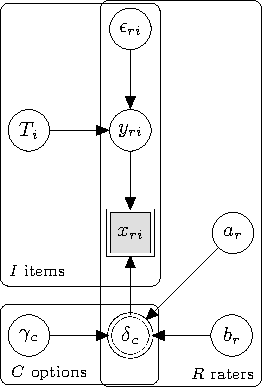
\includegraphics[width=\textwidth, page=1]{graphicalModels/graphicalModels.pdf}
		%	\caption{cap1}
		%	\label{fig:img1}
		\end{minipage}\hfill
	\begin{minipage}{0.5\textwidth}
		{\large
		\begin{align*}
			x_{\Iitem\Irater} &\leftarrow 
			\begin{cases}
			1		& \text{if } y_{\Iitem\Irater} \leq \delta_{\Irater 1} \\
			\Incat	& \text{if } \delta_{\Irater, \Incat-1} < y_{\Iitem\Irater} \leq \delta_{\Irater\Incat} \\
			\Tncat	& \text{if } y_{\Iitem\Irater} > \delta_{\Irater \Tncat-1}
			\end{cases}\\
%			x_{\Irater\Iitem} &\sim OL(y_{\Irater\Iitem}, \delta_{\Irater\Incat})\\
			y_{\Irater\Iitem} &\leftarrow T_\Iitem + \epsilon_{\Irater\Iitem}\\
			\gamma_\Incat &\leftarrow \log(\Incat / \Tncat)\\
			\delta_{\Irater\Incat} &\leftarrow a_\Irater  \gamma_\Incat + b_\Irater\\
			T_\Iitem &\sim \dnorm{0}{1}\\
			\epsilon_{\Irater\Iitem} &\sim \dnorm{0}{\sigma^\epsilon_\Irater} \\
			\sigma^\epsilon_\Irater &\sim \dgamma{0.01}{0.01} \\
			a_\Irater &\sim \dgamma{0.01}{0.01} \\
			b_\Irater &\sim \dgamma{0.01}{0.01}
		\end{align*}
		}%
	\end{minipage}
	\caption{Graphical model corresponding to a CCT model for a single patient. Gray nodes are observed whereas white nodes are unobserved parameters. Square nodes are discrete and circular nodes are continuous. A double border implies that a node is ???.}
	\label{model:CCTO}
\end{figure}
%\DON{Er zijn twee manieren om het LTRM uit te leggen. I zoals Anders \& Batchelder, eerst het latente niveau en daarna naar de kans op de data. II Vanuit de kans op de data naar het latente niveau.}

The rating given by rater $\Irater$ on item $\Iitem$ is denoted $x_{\Irater\Iitem}$ and takes on discrete values from $1$ through $\Tncat$. \citeA{Anders2015cultural} formalize the core ideas of the LTRM with 6 axioms. There is a latent, shared cultural truth among the raters, which is captured by the item location parameters $T_\Iitem$ (Axiom 1). Since raters are not perfect measurement instruments, they draw a noisy version of the cultural truth for each item, called a latent appraisal and defined as $y_{\Iitem\Irater} = T_\Iitem + \epsilon_{\Irater\Iitem}$, where $\epsilon_{\Irater\Iitem}\sim \dnorm{0}{\sigma^\epsilon_{\Irater\Iitem}}$ (Axiom 2). The standard deviation of the appraisal error $\sigma^\epsilon_{\Irater\Iitem}$ reflects that raters differ in their precision, captured by $E_\Irater$, and that items differ in their difficulty, captured by $\lambda_\Irater$. These two components define the standard deviation, $\sigma^\epsilon_{\Irater\Iitem} = E_\Irater / \lambda_\Irater$ (Axiom 3). Latent appraisals are assumed to be conditionally independent given the latent truth $T_\Iitem$ and the appraisal error $\epsilon_{\Irater\Iitem}$ (Axiom 4). So far, the axioms describe a latent process that underlies each observation. To translate these latent appraisals to observed categorical responses, it is assumed that there exist $\Tncat - 1$ ordered thresholds $\delta_{\Irater\Incat}$, such that each $x_{\Iitem\Irater}$ is generated in the following way (Axiom 5):
\begin{align*}
	x_{\Iitem\Irater} = 
	\left\{\begin{array}{ll} 
	1		& \text{if } y_{\Iitem\Irater} \leq \delta_{\Irater 1} \\[4pt]
	\Incat	& \text{if } \delta_{\Irater, \Incat-1} < y_{\Iitem\Irater} \leq \delta_{\Irater\Incat} \\[4pt]
	\Tncat	& \text{if } y_{\Iitem\Irater} > \delta_{\Irater \Tncat-1}
	\end{array} \right.
\end{align*}
In practice the generating process of $x_{\Iitem\Irater}$ is probabilistic and described with an ordered logistic distribution\footnote{The choice for an ordered logistic distribution is arbitrary and an ordered probit distribution could also be used, as was done by \citeA{Anders2015cultural}.}, which gives:
\begin{align*}
%\text{OrderedLogistic}
P(x_{\Iitem\Irater}\mid y_{\Iitem\Irater},\delta_{\Irater}) = 
\left\{\begin{array}{ll} 
1 - \ilogit{y_{\Iitem\Irater} - \delta_{\Irater 1}}         & \text{if } x_{\Iitem\Irater} = 1, \\[4pt]
\ilogit{y_{\Iitem\Irater} - \delta_{\Irater,\Incat-1}} - 
\ilogit{y_{\Iitem\Irater} - \delta_{\Irater,\Incat}}         & \text{if } 1 < x_{\Iitem\Irater} < \Tncat,\\[4pt]
\ilogit{y_{\Iitem\Irater} - \delta_{\Irater,\Tncat-1}}       & \text{if } x_{\Iitem\Irater} = \Tncat. 
\end{array} \right.
\end{align*}
The thresholds $\delta_{\Irater\Incat}$ are not fixed across raters, but accommodate the response biases of the raters. \citeA{Anders2015cultural} do so by estimating $\Tncat-1$ ordered thresholds $\gamma$ and defining $\delta_{\Irater\Incat} = a_\Incat \gamma_\Incat + b_\Incat$ (Axiom 6). A technical difficulty of estimating $\Tncat-1$ is that the number of thresholds $\delta_{\Irater\Incat}$ increases with the number of response options. This introduces a large number of parameters that can be difficult to estimate, in particular when some response options are not observed. Instead of modeling each threshold individually, the thresholds can be described as deviances from an initial guess. This initial guess is $\ilogit{c/C}$. This yields a set of thresholds such that if the latent appraisal is 0 then $P(x_{\Iitem\Irater})$ is uniform. Using two rater specific parameters, a scale parameter $a_\Irater$ and a shift parameter $b_\Irater$, this initial uniform distribution can vary across raters. The response biases are incorporated in the same manner: $\delta_{\Irater\Incat} = a_\Irater\ilogit{c/C} + b_\Irater$. This translation of thresholds is called the Linear in Log Odds function and is a useful tool for parsimonious estimation of thresholds underlying ordinal data \cite{Fox1995, Gonzalez1999}.

An intuition for how the ordered logistic distribution can model different data sets is given in Figure~\ref{fig:orderedLogistic}. 

%Here, we adopt the approach 
%Not all raters are equally precise and not all items are equally easy to measure. This is captured by $\tau_{\Irater\Iitem}$
%
%(Axiom 3)
%
%
%
%To formally introduce the LTRM, the rating given by rater $\Irater$ on item $\Iitem$ is denoted $x_{\Irater\Iitem}$, and can take on discrete values from $1$ through $\Tncat$. %The discrete outcomes are the result of categorizing a continuous appraisal $y_{\Iitem\Irater}$ using a set of thresholds $\delta_{\Irater\Incat}$. 
%The realization of $x_{\Iitem\Irater}$ is assumed to follow an ordered logistic distribution\footnote{The choice for an ordered logistic distribution is arbitrary and an ordered probit distribution could also be used, as was done by \citeA{Anders2015cultural}.} with location $y_{\Iitem\Irater}$ and thresholds $\delta_{\Irater\Incat}$:
%
%\begin{align*}
%%\text{OrderedLogistic}
%P(x_{\Iitem\Irater}\mid y_{\Iitem\Irater},\delta_{\Irater}) = 
%\left\{\begin{array}{ll} 
%	1 - \ilogit{y_{\Iitem\Irater} - \delta_{\Irater 1}}         & \text{if } x_{\Iitem\Irater} = 1, \\[4pt]
%	\ilogit{y_{\Iitem\Irater} - \delta_{\Irater,\Incat-1}} - 
%	\ilogit{y_{\Iitem\Irater} - \delta_{\Irater,\Incat}}         & \text{if } 1 < x_{\Iitem\Irater} < \Tncat,\\[4pt]
%	\ilogit{y_{\Iitem\Irater} - \delta_{\Irater,\Tncat-1}}       & \text{if } x_{\Iitem\Irater} = \Tncat. 
%\end{array} \right.
%\end{align*}
%The ordered logistic distribution uses $\Tncat - 1$ thresholds to assign each of the $\Tncat$ outcomes a probability. This probability is equal to the area between subsequent thresholds for a logistic distribution, as illustrated in Figure~\ref{fig:orderedLogistic}.
\begin{figure}[!ht]
	\centering
	\begin{subfigure}{.5\textwidth}
		\centering
		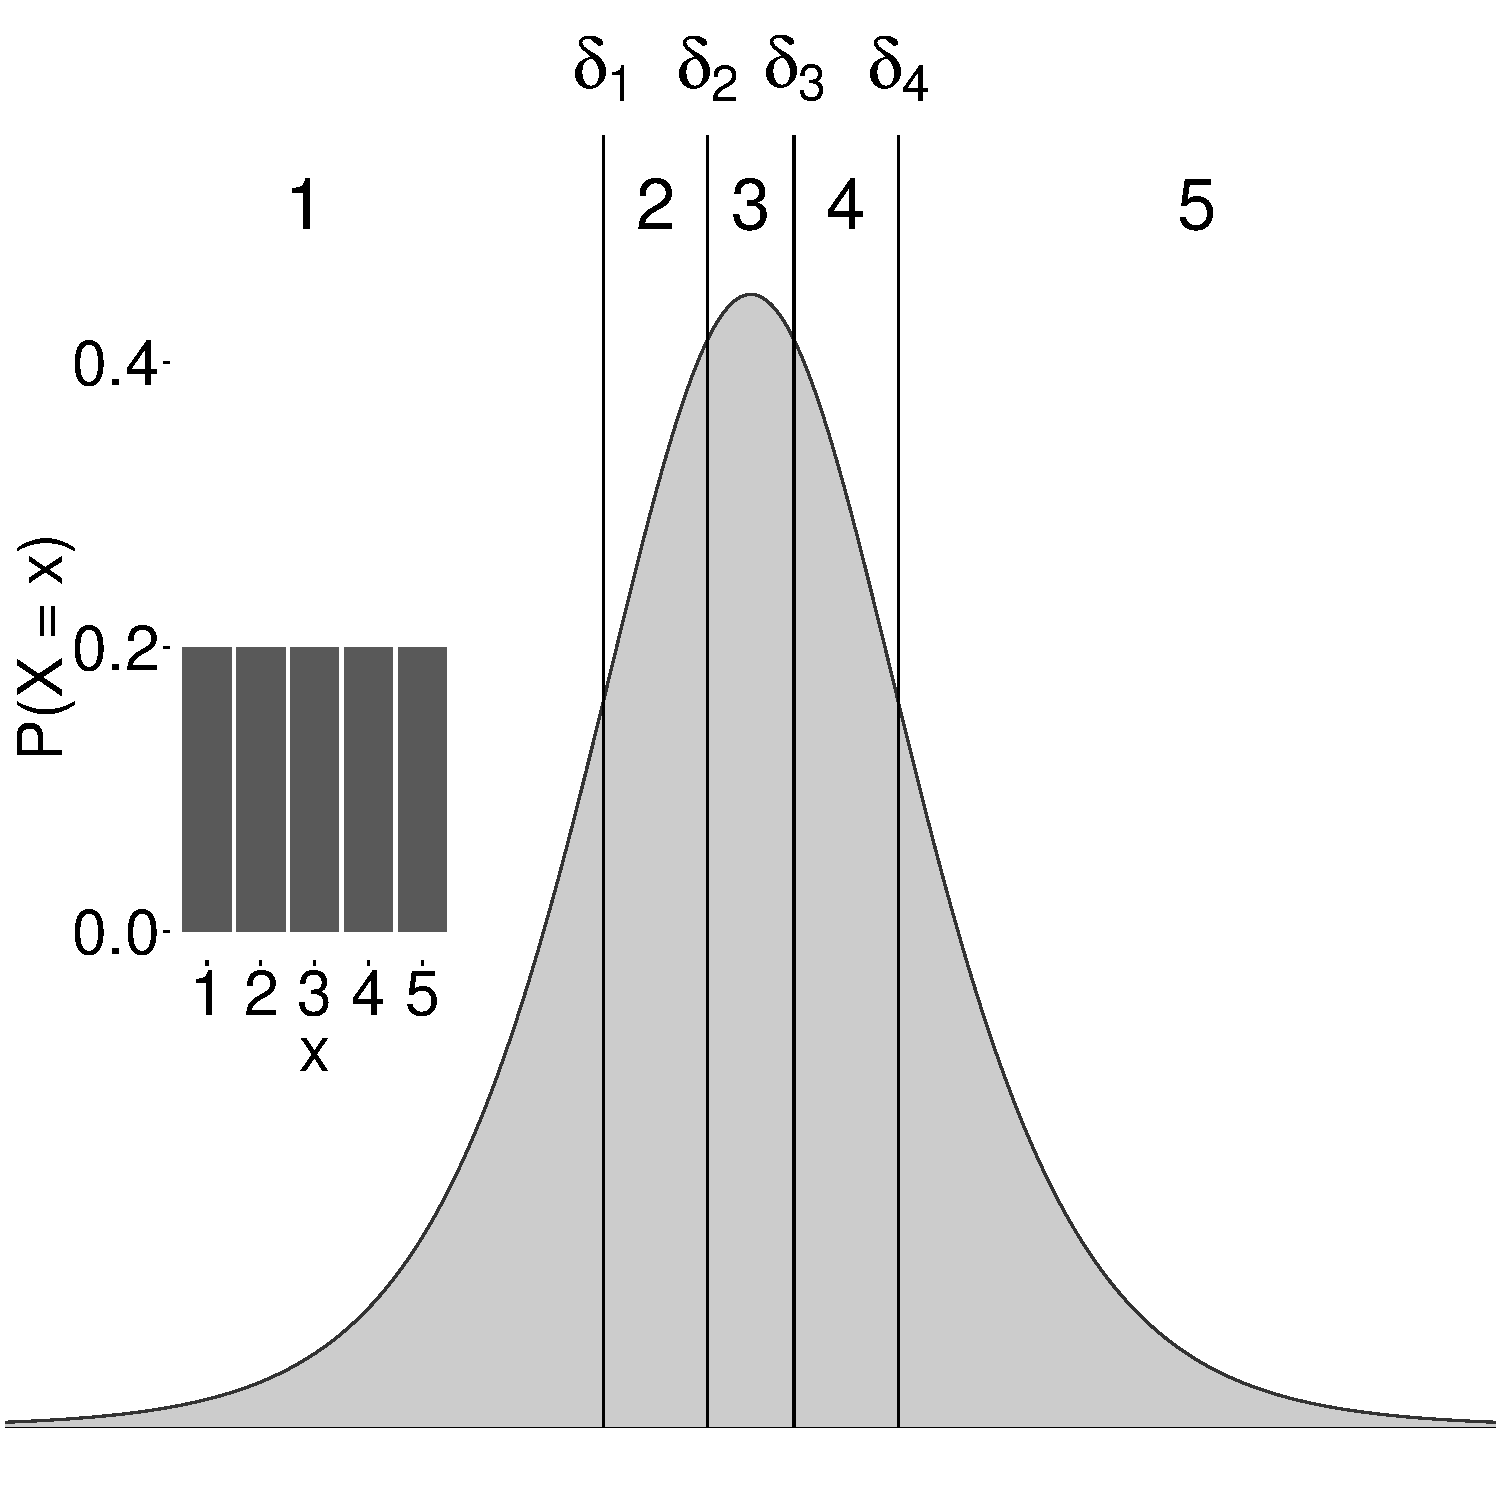
\includegraphics[width=.98\textwidth]{figures/orderedLogisticUnbiased.pdf}
%		\caption{A subfigure}
%		\label{fig:sub1}
	\end{subfigure}%
	\begin{subfigure}{.5\textwidth}
		\centering
		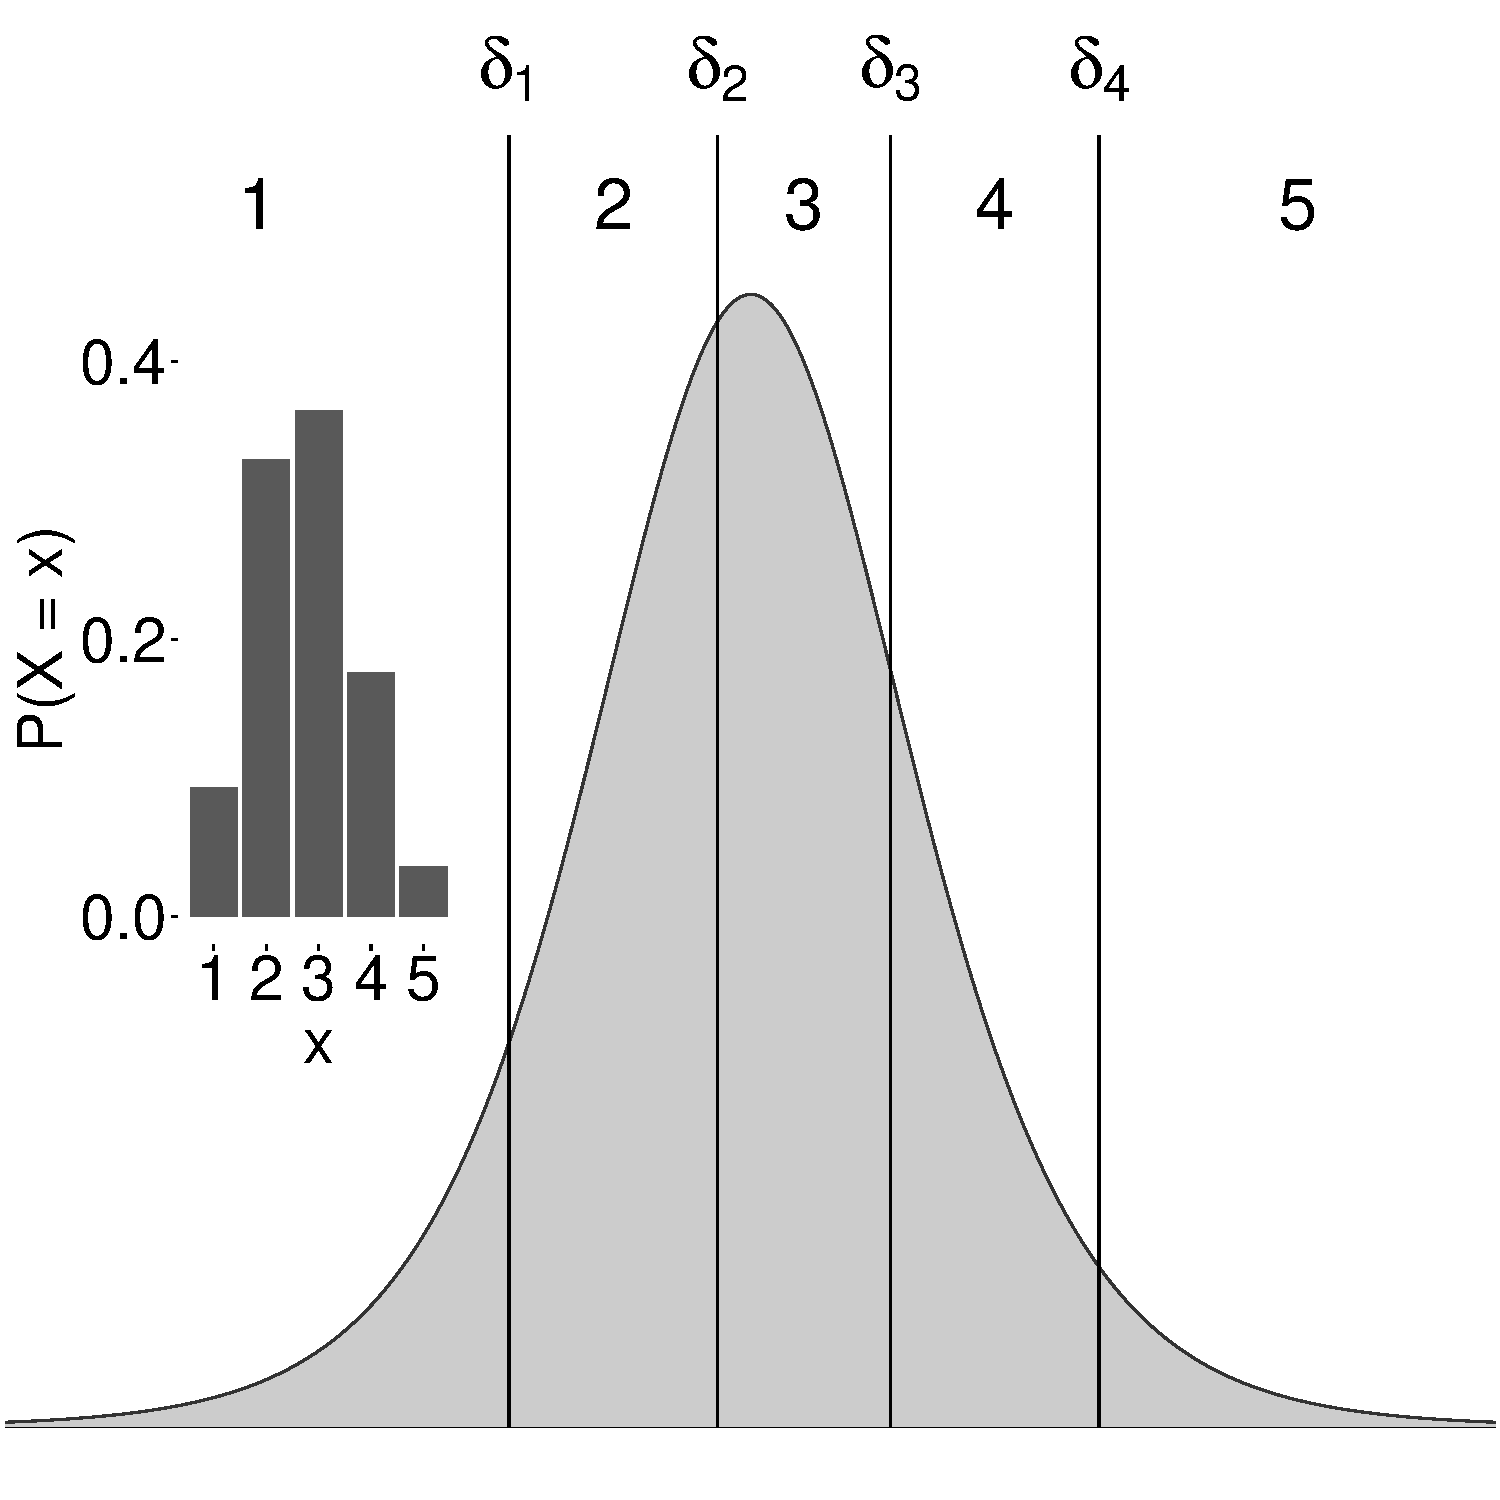
\includegraphics[width=.98\textwidth]{figures/orderedLogisticBiased.pdf}
%		\caption{A subfigure}
%		\label{fig:sub2}
	\end{subfigure}
	\caption{Ordered Logistic Distribution for $y_{\Iitem\Irater} = 0$ and varying thresholds. The implied probability distribution over categories is shown inside each panel. In the left panel, the thresholds are unbiased, $\alpha_\Irater = 1$, $\beta_\Irater = 0$. As a consequence, the distribution over outcomes is uniform. In the right panel, the thresholds are shifted right and the scale increased slightly, $\alpha_\Irater = 2$, $\beta_\Irater = 0.5$. The distribution over outcomes has most mass on outcomes 2 and 3.}
	\label{fig:orderedLogistic}
\end{figure}
%\DON{Als ik zo naar het model kijk vraag ik me af waarom we de bias in de latent appraisal nodig hebben, en of deze niet al opgevangen wordt door de rater specifieke thresholds.} 
%The main purpose of the ordered logistic distribution is to relate the probability of a discrete outcome to a continuous latent appraisal $y_{\Iitem\Irater}$ which can subsequently be linked to patient, rater, and item characteristics. The LTRM contains two components that capture rater bias. First, since raters are not perfect measurement instruments, their appraisal of an item can be biased. Therefore the appraisal is the sum of two components, the latent truth of an item $T_\Iitem$ and a residual of the rater for that item $\epsilon_{\Irater\Iitem}$. Second, the method by which an appraisal manifests a discrete realization can vary across raters. This is captured by the thresholds $\delta_{\Irater\Incat}$, which vary across raters. Modeling these sources of rater bias is of key interest because 
%
%we are interested in the consensus across raters for a particular item. This consensus is captured by latent truth of an item $T_\Iitem$.
%
%\DON{Anders \& Batchelder modelleren de thresholds als normaal verdeelt en sorteren ze daarna. Het lijkt mij leuker/ makkelijker om de parsimonious aanpak te gebruiken.}
%
%A technical difficulty of models for ordinal data is that the number of thresholds $\delta_{\Irater\Incat}$ increases with the number of response options. This introduces a large number of parameters that can be difficult to estimate, in particular when some response options are not observed. Instead of modeling each threshold individually, the thresholds are described as deviance from an initial guess. This initial guess is $\ilogit{c/C}$. This yields a set of thresholds such that if the latent appraisal is 0 then $P(x_{\Iitem\Irater})$ is uniform. Using two rater specific parameters, a scale parameter $a_\Irater$ and a shift parameter $b_\Irater$, this initial uniform distribution can vary across raters. The thresholds then become $\delta_{\Irater\Incat} = a_\Irater\ilogit{c/C} + b_\Irater$. This translation of uniform thresholds is called the Linear in Log Odds function and is a useful tool for parsimonious estimation of thresholds underlying ordinal data \cite{Fox1995, Gonzalez1999}.

The likelihood of the LTRM model is given by
\DON{willen we dit laten zien? Batchelder deed dit wel altijd.}


%The LTRM is an sophisticated model for data from multiple raters and . In the next section, 

The next step is to extend the LTRM model to describe multiple patients. In addition, we are often not just interested in the latent truth of an item, instead a group of items measure a construct. For instance, multiple items may be indicators of the underlying construct aggressiveness. Adding these two concepts to the LTRM model results in the graphical model shown in Figure~\ref{model:CCTO2}.
\begin{figure}[!ht]
	\centering
	\includegraphics[width=.6\textwidth, page=2]{graphicalModels/graphicalModels.pdf}
	\caption{Graphical model corresponding to the CCT model for a multiple patients.}
	\label{model:CCTO2}
\end{figure}



Add covariates for patients and raters.
\begin{figure}[!ht]
	\centering
	\includegraphics[width=.6\textwidth, page=3]{graphicalModels/graphicalModels.pdf}
	\caption{Graphical model corresponding to the CCT model for a single patient.}
	\label{model:CCTO3}
\end{figure}
 
 
 

The appraisals consists of the latent truth $T_\Iitem$ for each item and the bias of each rater $\epsilon_\Irater$. The thresholds are obtained by shifting and rescaleing 


to estimate a potentially large number of thresholds instead of needing a parameter per threshold \cite{Fox1995, Gonzalez1999}.


\newpage


personen/ raters zijn gebiased. Kan niet alleen eigenschappen van de gedetineerden halen maar ook die van de raters.

Covariaat voor e.g., hulpverleners versus psychiaters. Meerdere groepen raters (fixed effect).

Hierachisch niveau over patienten.

Covariaat voor groepen gedetineerden (fixed effect misdrijf).
Ofwel order restrictie voor deze groepen.

Missing values?

Hoe combineren we verschillende schalen van items?

kaart van hoe ontwikkelt zich dit over de tijd (zie figuur in proposal)

TODO: change model in NWO proposal to mimic SDT approach.

\section*{Simulation Results}

The sections below illustrate the use  

In all simulations, data was simulated using R \cite{R} and the posterior samples were obtained using Stan \cite{CarpenterEtAl2017Stan}. R files and Stan models are available in the online appendix at \osflink{}.

\subsection*{Parameter Retrieval}
Before interpreting or comparing a model, it is key to assess if its parameters can be accurately retrieved. For this purpose, we simulated a data set of 100 patients, 50 raters, 20 items, and 5 answer categories. A patient specific covariate containing five levels was added to mimic the effect of criminal offense. Similarly, three different categories of raters were assumed, which was also captured as a covariate.

\subsection*{Progress Monitoring}

\begin{figure}[!ht]
	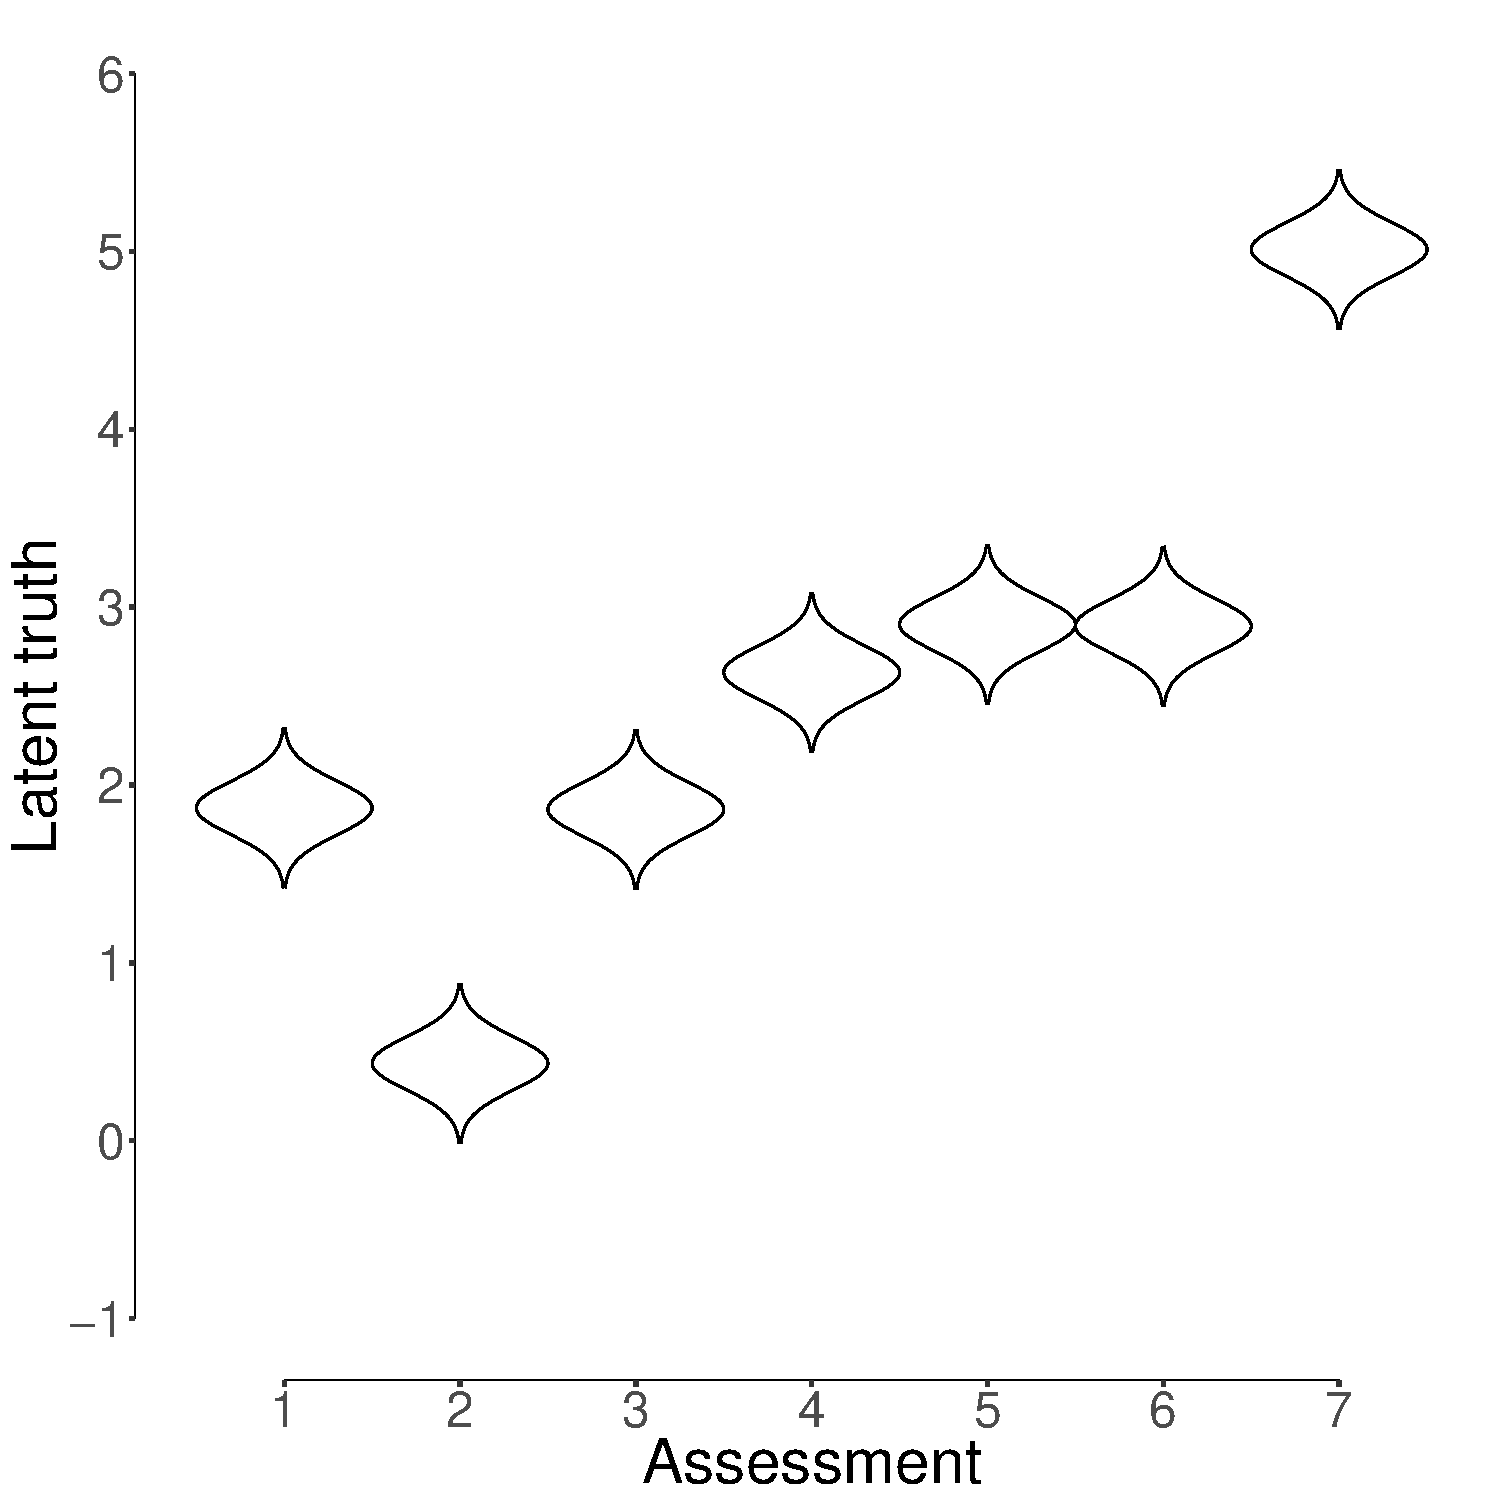
\includegraphics[width=\linewidth]{figures/progressMonitoring.pdf}
\end{figure}

\subsection*{Predictive Performance}

\section*{Discussion}


A common application of CCT is testing for multiple consensus truths.

\subsection*{Limitations}

Aanbeveling voor de praktijk

Bijhouden van evaluaties (scores + rater), liefst met hoge frequentie. 
Reden waarom iemand opgesloten is (reason of incarceration).
zo min mogelijk missing not at random.
``handig'': training in invullen om verschillen tussen raters te minimalizeren.
(V)AR component?

\bibliographystyle{apacite}
\bibliography{references}

\end{document}
